%#!platex
% NLP2024 サンプル文書.パブリックドメイン.
\documentclass[
  platex, dvipdfmx,  % ワークフローは必ず明示的に指定する
]{nlp2024}
%english option
%\documentclass[platex, dvipdfmx, english]{nlp2024}
%#!uplatex
%\documentclass[uplatex,dvipdfmx]{nlp2024}
%#!lualatex
%\documentclass[lualatex]{nlp2024}


% パッケージ
\usepackage{graphicx,xcolor}  % グラフィックス関連
\usepackage{pxrubrica}        % ルビ
\usepackage{url}
\usepackage{here}
\usepackage{enumitem}
%% option 不要な場合はコメントアウト
%\usepackage{jlreq-deluxe}     % 多書体化(otf パッケージは使用しない)
\usepackage{bxjalipsum}       % ダミーテキスト
\usepackage{hyperref}
\hypersetup{
	colorlinks=true, 
    citecolor=blue, 
    linkcolor=blue,
    urlcolor=blue,
	pdfborder={0 0 0},
}
\usepackage[verb]{bxghost}    % \verb 前後に適切な和欧文間スペース

% 参考文献のフォントサイズを指定
%\renewcommand{\bibfont}{\normalsize} % 標準サイズ
%\renewcommand{\bibfont}{\footnotesize} % より小さく

% \emph をゴシックかつ太字に(比較的新しい LaTeX が必要)
\DeclareEmphSequence{\gtfamily\sffamily\bfseries}

% 著者用マクロをここに入れる
\newcommand{\pkg}[1]{\textsf{#1}}
\newcommand{\code}[1]{\texttt{#1}}
\newcommand{\comment}[1]{\textcolor{red}{#1}}
%%%%%%%


\title{レビューの多角的な有用性判別のための分析と分類モデルの構築}

\author{%
  屋比久博文${}^{1}$ 當間愛晃${}^{2}$ \\
${}^{1}$琉球大学大学院 理工学研究科 知能情報プログラム\\
 ${}^{2}$琉球大学工学部工学科知能情報コース\\
  \texttt{k238571@ie.u-ryukyu.ac.jp}
 \texttt{tnal@ie.u-ryukyu.ac.jp}\\}

\begin{document}

\maketitle
\begin{abstract}
%NLP2022より,読者の論文理解を促進するため,所定のフォーマットの一部として投稿論文の概要を記載することにした(NLP2021までは概要は記載する必要がなく,ほぼ全ての論文で概要が存在しなかった).
%分量の目安は日本語/英語ともに「8〜13行」とする.概要が8〜13行を満たさなくても賞選考対象外や不採択になることはない.ただし,極端に短い/長い概要にならないように留意すること.
%日本語の場合は,文書クラスにより一行23文字に設定されているため,161文字から299文字相当になる.
多角的な有用性判別の実現を目的としてECサイトのレビュー体系分析を行った.分析の結果,レビューの傾向は「日常的に利用する商品」と「一時的に利用する商品」で異なることがわかった.「日常的に利用する商品」に焦点をあてさらに分析することで9つのラベルを考案し,各ラベルに自動で分類するモデルの構築と精度向上のための3つのパターンで実験を行った.その結果,損失関数の重み調整が精度向上に寄与することが確認された.分類精度の更なる改善に向けて,オーギュメンテーション,不均衡データになりづらいラベル設計や交差検証の検討が必要であると考えている.

\end{abstract}

\section{はじめに}
インターネットの普及により商品を購入する際,SNSやレビューサイトを利用して商品情報を収集する人が増加している.さらにオンラインショッピングサイトであるAmazon\footnote{https://www.amazon.com/}や楽天\footnote{https://www.rakuten.com/}の登場によりその利用者と商品に対するレビューもまた増加傾向にある.しかし,膨大なレビューのすべてに目を通し,必要なレビューを収集することはユーザーにとって大きな負担となる.

この問題に対して,「Amazonレビュー文の有用性判別実験\cite{Article_02}」や「有用なレビューを抽出するための比較文フィルタリングの検討\cite{Article_03}」のようにレビュー文がユーザーにとって有用であるかを判別する研究は多く行われている.これらの研究では「購入するかどうかの意思決定に寄与する文を,ユーザーにとって有用な文」と位置付け,各ユーザーの趣味趣向を考慮しない,
有用であるかどうかの2値分類を行っている.

また,Hongらは有用性であるかどうかの決定要因は,一貫性がなく有用性の測定法,レビュープラットホーム,製品タイプの3つの要因によって異なると主張している\cite{Article_04}.このように有用性の基準については多く議論されており,様々な観点から有用性を評価する研究なども行われている.

曽田らが行った「商品レビューの複数の観点からの有用性の評価\cite{Article_05}」では有用性を「評価表現に対する根拠がある」,「商品に関係のある言及が多い」,「他の商品と比較している」,「実際に商品を使用した(あるいはしていない)と推測できる」,「評価(レーティング)に対する根拠がある」,「文量が多い」,「文章が読みやすい」といった7つの観点に分類し,前者3つの観点の評価を実現した.しかし,有用性の様々な視点からの評価という面においては実現できている3つの観点では不十分であると言える.例えば,「商品に関係のある言及が多い」という観点で商品配送についてのレビューは除外されているが,ユーザーによってはこのレビューを重要視するケースも考えられる.また,「関係のある言及」がどのようなものか明瞭であるとユーザーにとってさらに多角的な評価となり有益である.

本研究では,多角的な有用性判別の実現を目的にECサイトのレビュー体系を分析し,先行研究\cite{Article_04, Article_05}の知見や消費者庁「消費者意識基本調査\cite{url1}」を踏まえ,レビューに付随するラベルの考案と付与を行った.また,考案したラベルを基に各カテゴリに自動で分類できるような自然言処理モデルの構築に取り組んだ.

\section{実験設計}

\subsection{ラベル考案}
\label{sec:contents-format1}
Amazonカスタマーレビューよりレビューを収集し,商品タイプによるレビュー傾向の違いを観察した.その結果,電化製品や日用品など継続的に利用する商品と映画やゲームなど一時的に利用する商品との間に異なるレビュー傾向が見られた.表\ref{table1}にそれぞれのタイプのレビュー例を示す.
\begin{table}[t]
  \caption{それぞれのタイプのレビュー例}
  \label{table1}
  %\scriptsize
  \centering
  \begin{tabular}{|l|l|}
    \hline
    & レビュー例 \\
    \hline
    ゲーム(ピクミン)    & 
    \begin{tabular}{p{4cm}}
    ピクミンは可愛いし内容も面白い。
他の皆さんが言ってるようにプレイ時間が短いので星4つ。
永遠に遊べるピクミン作って欲しいな。
    \end{tabular}\\
    \hline
    電化製品(掃除機)  & 
    \begin{tabular}{p{4cm}}
    吸引力もしっかりあり、コード付きなので使いたい時に充電器にせず使えていいですが音は大きめです
      \end{tabular}\\
    \hline
    \end{tabular}
\end{table}


ゲームのレビューでは「面白い」や「楽しい」といった一時的な感情表現を用いて評価をする傾向が見られるのに対して,電化製品のレビューでは機能面での実用性を述べる日常的に利用することを前提とした評価をする傾向が見られた.この分析より本研究では商品タイプを「一時的に利用する商品」と「日常的に利用する商品」という2タイプに分けることとし,これらに付随するレビューの傾向が異なると仮定した.また上記2タイプの各商品には「商品内容に触れた評価レビュー」,「商品内容に触れない評価レビュー」,「評価をしていないもの」の3タイプのレビューが見られ,この3タイプのレビューをさらに細分化したレビューの評価基準をラベルとした.なお今回は「日常的に利用する商品」に着目してレビューを収集した.レビューの体系を図\ref{fig1}に示す.

\begin{figure}[t]
\centering
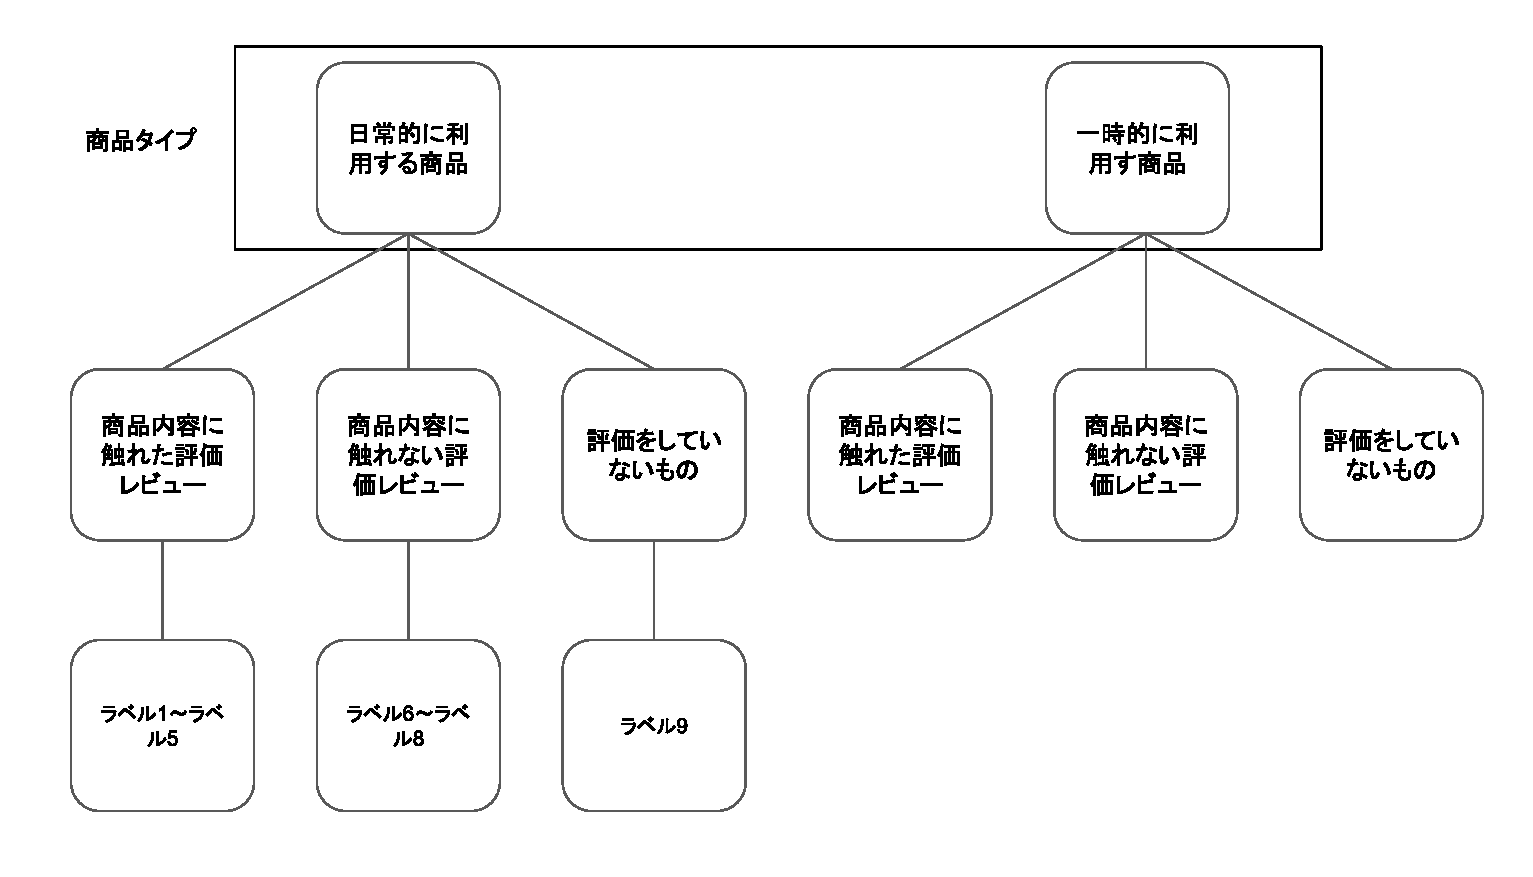
\includegraphics[width=8.5cm]{review-fig.eps}
\caption{レビュー体系図}
\label{fig1}
\end{figure}


考案したラベルを以下に示す.
\paragraph{ラベル1} 商品機能に触れたレビュー\\
商品のサイズや性能面についての言及を含むレビューがこのラベルに該当する.\\
\emph{レビュー例}:
風量は思ったより強いですが、音も静かだし、プラズマクラスターだし気に入っています。\\

\paragraph{ラベル2} 別の商品内容のレビュー\\
レビュー元の商品から逸脱し,別の商品の解説を行なっているレビューがこのラベルに該当する.\\
\emph{レビュー例}:
最近買ったホームセンター製の扇風機が買って2年ほどで廻らなくなりました。
やはり国内メーカーの製品が良いかな\\

\paragraph{ラベル3} 別の商品との比較を交えたレビュー\\
レビュー元の商品と別の商品の比較を交えて評価しているレビューがこのラベルに該当する.以下のレビュー例はラベル1と3の複合型となっている.\\
\emph{レビュー例}:扇風機って長持ちするから、20年前の物との比較ですが、
静か、梱包がコンパクト、組立簡単でした。
また20年持つのかな?\\
\paragraph{ラベル4} 商品価格に触れたレビュー\\
商品の価格表現(安い,高い,コスパ等)を含むレビューがこのラベルに該当する.\\
\emph{レビュー例}:各部屋にコスパよし\\
\paragraph{ラベル5} ユースケースを述べたレビュー\\
商品の活用例や体験談を交えて評価をしているレビューがこのラベルに該当する.以下のレビュー例はラベル1と5の複合型となっている.\\
\emph{レビュー例}:静粛性は抜群で 熱帯夜の夜は エアコンとの合わせ技で大活躍でした。
表示関係も派手じゃないので 夜間まぶしいこともなく 良かったです。
強いてあげれば あまりにも重いのが難点で 掃除の時に場所をずらすのが
ちょっと気合いが筆世です。\\
\paragraph{ラベル6} 簡易的な感想表現のみのレビュー\\
商品内容に触れず,良し悪しのみで評価するレビューがこのラベルに該当する.\\
\emph{レビュー例}:心地よい。\\

\paragraph{ラベル7} 商品状態に触れたレビュー\\
商品の配送時に生じる商品状態の変化や中古品の保存状態を評価したレビューがこのラベルに該当する.\\
\emph{レビュー例}:傷がついていた事以外は機能面に問題はなし。
しかし、外装もしょうひんではと、、、\\
\paragraph{ラベル8} 配送条件に触れたレビュー\\
商品配送期間や商品配送時のサービスを評価したレビューがこのラベルに該当する.\\
\emph{レビュー例}:注文した翌日には商品が届きました。よい買い物をさせていただきました。\\
\paragraph{ラベル9} 批評をしていないもの\\
批評を行なっておらず,レビューとは言い難いものがこのラベルに該当する.\\
\emph{レビュー例}:特にありません。\\
\subsection{実験手順}
本実験ではBERT\cite{Article_06}を用いたファインチューニングによってマルチラベル分類モデルの構築を行った.
行った3パターンの実験を以下に示す.
\begin{description}
 \item[パターン1] 100件のレビューに対し9つのラベルを付与しマルチラベル分類を行う.
 \item[パターン2] 766件のレビューに対し9つのラベルを付与しマルチラベル分類を行う.
 \item[パターン3] パターン2の分類をベースに全データの合計数と各ラベルの比率に応じた重みを加えたマルチラベル分類を行う.
\end{description}

実験手順の詳細を以下に示す.
\begin{itemize}
  \item 1つの商品から収集した100件のレビューをパターン1のデータ,さらに追加した7つの商品レビューを合計した766件のレビューをパターン2とパターン3のデータとした.
  \item \ref{sec:contents-format1}節で定義したラベルを基にアノテーションを行い,データセットを構築する.
  \item データセットをtrain : val : test = 6 : 2 : 2 の割合で分割する.学習率は1e-6とし,maxエポックは50で10エポックのうち検証データに対する損失が改善されない場合,学習を終了する条件を加えた.
  \item 事前学習済み日本語BERTモデル(`cl-tohoku/bert-base-japanesewhole-word-masking')を基にファインチューニングを行う.
\end{itemize}

パターン3では上記に加えて以下の設定を行った.
\begin{itemize}
  \item 全データ数に対する各ラベルの逆比に0.4を乗算したものを重みとして設定した.0.4という数値は,パターン2の重みデフォルト値が1であるのに対して逆比が大きくなりすぎることから,スケールを縮小するため著者が直感的に設定したものである.式は以下のようになる.\\
  \begin{equation}
 	各ラベルの重み = \frac{全データ数766件}{各ラベル数} \times 0.4
 \end{equation}
\end{itemize}
\subsection{評価手法}
本研究では分類学習の評価手法として多く利用されているaccuracy,recall,precision,f1 score を指標に分類結果の指標とした.
%\ref{sec:contents-format1}節および\ref{sec:contents-format2}節に詳述する.





\section{実験結果と考察}
%\label{sec:contents-format1}
表\ref{table2}にパターン1,表\ref{table3}にパターン2,表\ref{table4}にパターン3のtestデータにおける分類結果を示す.それぞれの表は各ラベル(testラベル数 / train,val,testラベルの総数)という形式である.また各ラベル毎のaccuracy,recall,precision,f1scoreにおける値が0以外のベストスコアは強調表示している.
\begin{table}[t]
  \caption{100件のレビューで学習した分類結果(パターン1)}
  \label{table2}
  %\scriptsize
  \centering
  \small
  \begin{tabular}{|l|l|l|l|l|}
    \hline
    \small
    \begin{tabular}{p{2.2cm}}
    ラベル種別(該当レビュー数/各ラベル毎の総数)
    \end{tabular}
    & accuracy & recall & precision & f1score \\
    \hline
    ラベル1 (15/68)   & 0.79 & \emph{1.00} & 0.79 & 0.88 \\
    \hline
    ラベル2 (0/0)  & \emph{1.00} & 0.00 & 0.00 & 0.00 \\
    \hline
    ラベル3 (1/2)  & \emph{0.95} & 0.00 & 0.00 & 0.00 \\
    \hline
    ラベル4 (5/22)  & 0.68 & 0.00 & 0.00 & 0.00 \\
    \hline
    ラベル5 (13/52)   & 0.63 & \emph{0.92} & \emph{0.67} & \emph{0.78} \\
    \hline
    ラベル6 (0/6)   & 0.95 & 0.00 & 0.00 & 0.00 \\
    \hline
    ラベル7 (0/6)  & \emph{0.95} & 0.00 & 0.00 & 0.00 \\
    \hline
    ラベル8 (1/4)   & 0.89 & 0.00 & 0.00 & 0.00 \\
    \hline
    ラベル9 (0/0)   & 1.00 & 0.00 & 0.00 & 0.00 \\
    \hline
    \end{tabular}
\end{table}

\begin{table}[t]
  \caption{766件のレビューで学習した分類結果(パターン2)}
  \label{table3}
  %\scriptsize
  \small
  \centering
  \begin{tabular}{|l|l|l|l|l|}
    \hline
    \begin{tabular}{p{2.2cm}}
    ラベル種別(該当レビュー数/各ラベル毎の総数)
    \end{tabular}
    & accuracy & recall & precision & f1score \\
    \hline
    ラベル1 (136/660)   & \emph{0.88}  & \emph{1.00}       & \emph{0.88}         & \emph{0.94}\\
    \hline
    ラベル2 (0/2)  & \emph{1.00}  & 0.00       & 0.00         & 0.00\\
    \hline
    ラベル3 (27/88)   & 0.82  & 0.00       & 0.00         & 0.00\\
    \hline
    ラベル4 (34/154) & 0.76  & 0.00       & 0.00         & 0.00\\
    \hline
    ラベル5 (62/231)  & \emph{0.60}  & 0.02       & 0.33         & 0.07\\
    \hline
    ラベル6 (5/32)  & \emph{0.97}  & 0.00       & 0.00         & 0.00\\
    \hline
    ラベル7 (8/20)  & \emph{0.95}  & 0.00       & 0.00         & 0.00\\
    \hline
    ラベル8 (10/19)  & 0.94  & 0.00       & 0.00         & 0.00\\
    \hline
    ラベル9 (3/18)  & 0.98  & 0.00       & 0.00         & 0.00\\
    \hline
    \end{tabular}
\end{table}

\begin{table}[t]
  \caption{766件のレビューと各ラベルに重みを加えて学習した分類結果(パターン3)}
  \label{table4}
  \small
  %\scriptsize
  \centering
  \begin{tabular}{|l|l|l|l|l|}
    \hline
    \begin{tabular}{p{2.2cm}}
    ラベル種別(該当レビュー数/各ラベル毎の総数)
    \end{tabular}
    & accuracy & recall & precision & f1score \\
    \hline
    ラベル1 (133/660)   & 0.86  & \emph{1.00}       & 0.86         & 0.92\\
    \hline
    ラベル2 (0/2) & \emph{1.00}  & 0.00       & 0.00         & 0.00\\
    \hline
    ラベル3 (23/88)  & 0.76  & \emph{0.35}       & \emph{0.27}         & \emph{0.30}\\
    \hline
    ラベル4 (33/154) & \emph{0.79}  & 0.00       & 0.00         & 0.00\\
    \hline
    ラベル5 (67/231)  & 0.49  & 0.73       & 0.45         & 0.56\\
    \hline
    ラベル6 (8/32)  & 0.95  & 0.00       & 0.00         & 0.00\\
    \hline
    ラベル7 (10/20)  & 0.92  & 0.00       & 0.00         & 0.00\\
    \hline
    ラベル8 (7/19)  & \emph{0.95}  & 0.00       & 0.00         & 0.00\\
    \hline
    ラベル9 (0/18)  & \emph{1.00}  & 0.00       & 0.00         & 0.00\\
    \hline
    \end{tabular}
\end{table}

\subsection{パターン1とパターン2の比較}
\label{sec:contents-format2}
表\ref{table2}および表\ref{table3}に注目して観察すると,比較的全データ数における割合が大きいラベル1では2つのパターンで高い値を取っている.また,データ数の増加によってラベル5のaccuracy,recall,precision,f1 scoreともに数値が減少していることがわかる.この数値の低下は,パターン1においてラベル5が全データの約50%を占める一方で,パターン2ではその割合が30%に減少していることに起因していると考えられる.

上述のことから分類モデルにおける各ラベルの損失を調整することや各ラベル数と全データ数との均衡を保つことが精度改善につながると言える.


\subsection{パターン2とパターン3の比較}
表\ref{table3}および表\ref{table4}に注目して観察すると,重みを調整したことによりラベル3とラベル5における評価の値に改善が見られる.このことから節\ref{sec:contents-format2}で述べた損失を調整することによりモデルの性能向上に寄与する可能性を裏付けるものとなった.

ラベル2,6,7,8,9では精度の改善は見られなかった.ラベル2,7,8,9は節\ref{sec:contents-format2}で述べたように,全データ数に対する各データ数が極端に少ないことが主な要因となっており,ラベルの重み調整による改善は見込めないと考えている.少数ラベルに対する重みをさらに増加させた場合でも,ほぼ完全一致のレビューのみ判定するようになると考えられるためである.

こういった極端に少ないデータ数に講じる策としては,純粋に偏ったデータを増加させるオーギュメンテーション,損失関数の設計を見直す,人の価値観\cite{Article_07}を利用したラベル設計で不均衡データを避けることなどが考えられ,これらの手法について今後検討が必要であることがわかった.

ラベル6は少数ということの他に,valとtestに割り当てられたデータ数が起因していることも考えられる.こちらは交差検証を行うことで再度検証.

また,ラベル4についてはラベル3と比較してデータ数が多いにも関わらず評価が改善できなかった.現状この問題について分析できておらず検討の必要がある.


\section{まとめと今後の課題}
Amazonレビュー文の分析を行い体系化を試みた.レビュー文は「一時的に利用する商品」と「継続的に利用する商品」の2つの商品タイプで傾向が異なることが確認できた.「日常的に利用する商品」の体系に基づいてレビュー文に対する分類ラベルを設計し,日本語BERTモデルを用いてファインチューニングを行った.各ラベルの重み調整によりモデルの性能改善が一部見込めるが,極端に少ないデータセットに対しては有効でないことがわかった.今後は対策としてオーギュメンテーションや損失関数の再設計,不均衡データになりづらいラベル設計などの手法を検討していく必要がある.また,「一時的に利用する商品」のレビュー収集を進め分類モデルの構築に取り組んでいきたい.





%%%%  ここまでが本文 4ページ以内
\clearpage


% 参考文献
\bibliographystyle{junsrt}%junsrt
\bibliography{jyourrefs} % ファイル名は適宜自分のbibファイルに置き換える

%%%%  ここまでが本文+参考文献 5ページ以内


% 付録(Appendix)
% 付録を付けない場合は,以下\end{document}以外を全てをコメントアウトする.
% 本文,参考文献に続けて作成する場合は,必ず \clearpage して新たなページとする
\clearpage
% 付録は別ツールで作成して,後で本文PDFに追加する方式でもよい
\appendix
% ここ以降はフォーマットを自由に変更可能
%\onecolumn % onecolumnにしたい時の例

%\small % 文字サイズを小さくする. 一行23文字 => 26文字




\end{document}
